\chapter{Desenvolupament d’un entorn IoMT simulat}
Per al desplegament d’un entorn IoMT simulat seguint l’arquitectura explicada a \ref{sec:Topologia} s'ha utilitzat dispositius reals (amb ordinadors convencionals i Raspberry Pi) i simulats a través de contenidors Docker i l’orquestrador Docker Compose.

Per a la realització dels clients, que representen el trànsit benigne, he utilitzat una imatge d’Ubuntu \cite{ubuntuimg}, aquesta ha estat modificada instal·lant l'eina \textit{mosquitto-clients 2.0.20}. Amb aquesta aplicació podem fer actuar aquest contenidor d'Ubuntu com un client MQTT i tenir les seves funcions principals com subscriure’s i publicar a un tòpic d’un broker concret i utilitzar totes les funcionalitats descrites a \ref{sec:mosquitto}. També he instal·lat Python 3.13.2 i Paho-mqtt 2.0.0 \cite{pahoexp} per a poder generar paquets de forma personalitzada. Amb aquesta llibreria de Python podem modificar aspectes molt més concrets de les nostres connexions MQTT i paquets, canviant els valors de les dades o la freqüència d’enviament de les publicacions. Gràcies a aquesta eina, al ser una llibreria de Python, podem córrer els clients de manera automatitzada mitjançant funcionalitats pròpies del llenguatge Python. Finalment, he instal·lat les eines net-tools i iputils per tal de poder monitoritzar l’estat dels contenidors i fer comprovacions de connectivitat.

Pel que fa al Broker, he utilitzat l’imatge oficial de mosquitto anomenada \textit{eclipse-mosquitto (versió 2.0.21)} \cite{mosquittoimg}. Aquesta permet l’ús del contenidor com a broker MQTT en les seves versions 3.1 i 5.1.1 amb totes les funcionalitats de les quals disposa la versió local. Respecte a la seva configuració de Docker, he mapejat els ports 1883 i 8883 perquè en establir una connexió TCP a un d’aquests ports de l'hipervisor es dirigeixi al mateix port del contenidor broker. També he generat 3 volums compartits amb l'hipervisor:
\begin{itemize}
    \item \textbf{Config:} on s’ubica el fitxer de configuracions mosquitto.conf
    \item \textbf{Data:} on opcionalment s'emmagatzemen les dades rebudes en format txt o dintre una base de dades
    \item \textbf{Log:} on es guarden els logs dels errors ocasionats durant el seu funcionament en fitxers .log
\end{itemize} 

Pel que fa al monitor de trànsit, partint de l’image base Ubuntu, s’ha instal·lat \textit{tcpdump 4.99.5} i \textit{wireshark 4.4.3} ( \ref{sec:TCPDump} ). Com ha estat explicat a \ref{sec:Topologia}, la seva funcionalitat és emmagatzemar el trànsit per tal de generar el dataset mitjançant \textit{tcpdump} i \textit{Wireshark}. Per tal de poder visualitzar l'interfície gràfica de Wirehark, s’ha fet servir el socket de X11 de l’hipervisor mapejat al contenidor.

Per l’atacant, parteix de la imatge \textit{kalilinux/kali-last-release} \cite{kaliimg} amb l’instal·lació dels paquets \textit{kali-linux-headless} que conté les eines més utilitzades de kali linux i depenent de l’atac s’ha instal·lat altres eines de pentesting explicades posteriorment.

Per al desplegament de contenidors per part de l'atacant, he configurat una xarxa personalitzada de docker mitjançant l'eina \textit{Docker Compose} on es disposen tots els contenidors i tenen connectivitat entre ells com si es tractés d'una xarxa LAN privada. 

Per integrar aquest desplegament en un model híbrd entre dispositius simulats i dispositius reals, s’ha utilitzat la configuració de xarxa dintre \textit{Docker Compose} anomenada \textit{MACVLAN} que permet connectar els contenidors a la xarxa física amb adreces IP i MAC diferent a la del hipervisor (cal evitar conflictes amb altres adreces ja utilitzades en xarxa física), amb un efecte similar al que tindríem connectant un switch a la xarxa amb tots els seus contenidors. Amb aquesta configuració m'he coordinat amb altres membres del grup ISG-UPC per a poder integrar el meu treball al projecte. 
Finalment, en diversos atacs, he configurat l'entorn amb el mode \textit{IPVLAN (L2)} on cada contenidor té una adreça IP diferent, però, l'hipervisor sobreposa la seva adreça MAC i respon a peticions ARP per a les diferents adreces IP. Això és mès compatible en xarxes WiFi WPA2.

 \begin{figure}[H]
    \centering
    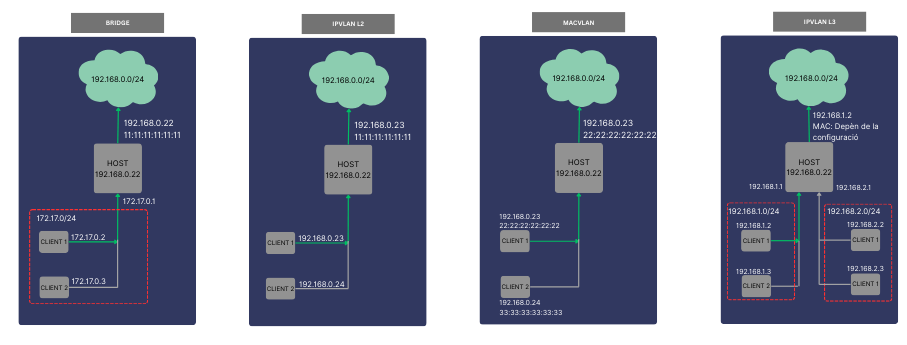
\includegraphics[width=1\textwidth]{img/DockerNetworks.png}
    \caption{La figura mostra el comportament dels diferents drivers de xarxa de Docker (excloent el mode host on directament actua en nom de l'hipervisor).}
    \label{fig:DockerNetworks}
  \end{figure}

Per concloure, per a l'execució dels diferents atacs explicats en aquest treball, es pot resumir l'estructura de xarxa seguint aquest esquema:

 \begin{figure}[H]
    \centering
    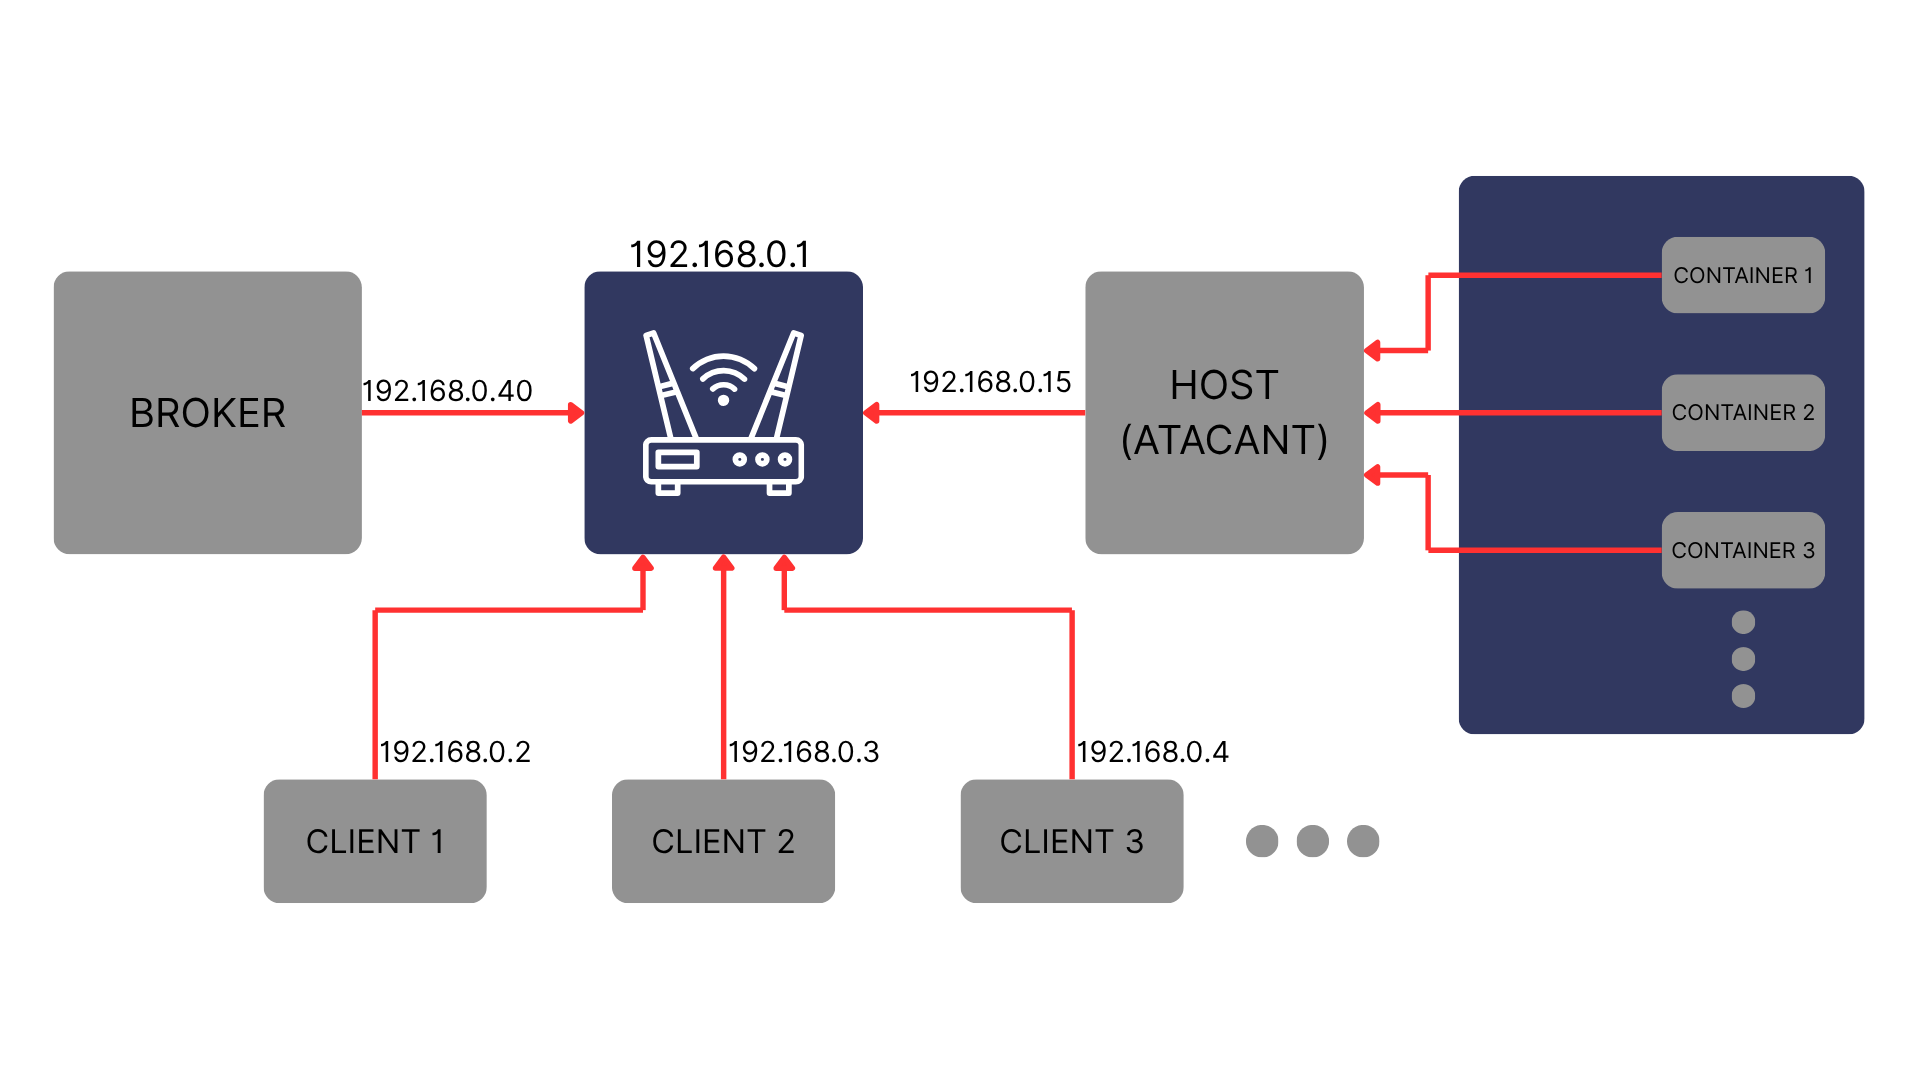
\includegraphics[width=1\textwidth]{img/infraXarxa.png}
    \caption{La figura mostra la infraestructura de xarxa dissenyada per als diferents atacs: Consta d'una xarxa Wifi amb un broker, un nombre varaible de clients i l'atacant on s'hi despleguen xarxes virtuals diferents per a cada atac.}
    \label{fig:Infraestructura}
  \end{figure}
